% Master's thesis — Milestone 3, 15 min, widescreen, minimalist design.
% Compile: pdflatex milestone3.tex   (run from presentation/milestone3/)
% Built on the milestone2 template; structured around the three review comments.
%
% ASSET STATUS (paths are relative to this file, i.e. ../../plots/...):
%   [READY]  ../../plots/milestone2/donor_importance_heatmap.png
%   [READY]  naive numbers below come from data/validation/naive_baseline_comparison.csv
%   [READY]  placebo / LOO numbers carried from milestone2 validation battery
%   [READY]  breakpoint numbers from data/validation/{bai_perron_relationship,hlt_trend_break}_*.csv
%   [READY]  ../../plots/milestone3/donors_<category>_side_by_side.png  (6 per-category panels)
%            -> regenerate via notebooks/08_Milestone3_Plots.ipynb (19-donor shared pool).
%
% NOTE: donor pool is 19 (not the 21 the milestone2 deck stated) -- confirmed against
%       data/validation/donor_importance_consensus.csv. Placebo N=20, p-floor 1/20=0.05.

\documentclass[aspectratio=169,11pt]{beamer}

% ===== Minimal theme (identical to milestone2) =====
\usetheme{default}
\usecolortheme{default}

\setbeamertemplate{navigation symbols}{}
\setbeamertemplate{headline}{}
\setbeamertemplate{itemize item}{\textbullet}
\setbeamertemplate{itemize subitem}{\textendash}
\setbeamertemplate{itemize subsubitem}{\textperiodcentered}

\setbeamertemplate{footline}{%
  \hspace*{\fill}\textcolor{gray}{\footnotesize\insertframenumber\,/\,\inserttotalframenumber}\hspace*{1em}\vspace*{0.5em}%
}

\setbeamercolor{frametitle}{fg=black,bg=white}
\setbeamerfont{frametitle}{size=\Large,series=\bfseries}
\setbeamertemplate{frametitle}{%
  \vspace{0.3em}%
  \insertframetitle\par%
  \vspace{0.15em}%
  {\color{black!20}\hrule height 0.4pt}%
  \vspace{0.6em}%
}

\setbeamerfont{title}{size=\LARGE,series=\bfseries}
\setbeamerfont{subtitle}{size=\large,series=\mdseries,shape=\itshape}
\setbeamerfont{author}{size=\normalsize}
\setbeamerfont{institute}{size=\small,shape=\itshape}
\setbeamercolor{title}{fg=black}
\setbeamercolor{subtitle}{fg=black!70}
\setbeamercolor{author}{fg=black}
\setbeamercolor{institute}{fg=black!60}

\setbeamercolor{normal text}{fg=black,bg=white}
\setbeamercolor{structure}{fg=black}

\usepackage{graphicx}
\usepackage{booktabs}
\usepackage{array}
\usepackage{amsmath}
\usepackage{xcolor}
\hypersetup{colorlinks=true,urlcolor=black,linkcolor=black}

\definecolor{accent}{HTML}{8B0000}
\definecolor{muted}{HTML}{777777}

\newcommand{\src}[1]{{\footnotesize\textcolor{muted}{(#1)}}}
\newcommand{\smalltext}[1]{{\footnotesize\textcolor{muted}{#1}}}
\newcommand{\hd}[1]{\textbf{#1}}

\title{The Brent-Price Causal Effect of the\\ 2026 Hormuz Disruption}
\subtitle{ }
\author{Cherryl Chico \and Nikoloz Darsalia \and Elvis Casco}
\institute{BSE, Data Science for Decision Making 2025--2026}
\date{}

\begin{document}

% =====================================================================
% TITLE
% =====================================================================
{\setbeamertemplate{footline}{}
\begin{frame}[plain]
  \vfill
  \begin{center}
    {\LARGE\bfseries The Brent-Price Causal Effect of the\\[0.2em] 2026 Hormuz Disruption}\\[0.8em]
    {\large\itshape A Synthetic Control Approach --- Milestone 3}\\[2.5em]
    {\normalsize Cherryl Chico \quad Nikoloz Darsalia \quad Elvis Casco}\\[0.3em]
    {\small\itshape\textcolor{muted}{BSE, Data Science for Decision Making 2025--2026}}
  \end{center}
  \vfill
\end{frame}
}

% =====================================================================
% 0. Feedback from last presentation
% =====================================================================
\begin{frame}{Where we left off}
  \vspace{0.6em}
  \hd{Major feedbacks:}
  \vspace{0.3em}
  \begin{enumerate}\setlength\itemsep{0.4em}
    \item[\textcolor{accent}{\hd{1}}] \hd{Stronger justification that the selected donors satisfy SUTVA} ---
      i.e.\ that no donor is itself contaminated by the treatment.
    \item[\textcolor{accent}{\hd{2}}] \hd{Economic interpretation of \emph{why the models behaved as they did}}
      during the treatment period 
    \item[\textcolor{accent}{\hd{3}}] \hd{Explore a naive counterfactual} --- show what the SCM machinery buys us
      over simpler baselines.
  \end{enumerate}

  \vspace{0.5em}
  \smalltext{Re suggested reading \hd{Ham \& Miratrix}: it concerns pre-trend
  identification for \emph{matching / difference-in-differences} designs, not synthetic control on a price
  series, so its specific machinery does not transfer to our setting}

\end{frame}

% =====================================================================
% COMMENT 1 --- SECTION DIVIDER + THE FILTERING QUESTION
% =====================================================================
\begin{frame}{Comment 1 --- donor selection and SUTVA}
  \footnotesize
  \hd{The selection question, asked of every candidate:}
  \vspace{0.3em}
  \begin{center}
  \fcolorbox{accent!50}{accent!5}{\begin{minipage}{0.93\textwidth}
    \vspace{0.25em}
    \begin{center}
      {\normalsize\itshape Does the asset \textcolor{accent}{co-move with Brent through common global factors},
      yet stay \textcolor{accent}{off the oil-supply / disruption path}?}\\[0.3em]
      {\footnotesize\textcolor{muted}{Yes to both $\rightarrow$ include. On the oil-supply / disruption path
      (chokepoint or Russia/Ukraine trade) $\rightarrow$ exclude (SUTVA).}}
    \end{center}
    \vspace{0.1em}
  \end{minipage}}
  \end{center}

  \vspace{1.0em}
  \hd{Two contamination channels to screen out:}
  \vspace{0.3em}
  \begin{itemize}\setlength\itemsep{0.5em}
    \item \hd{The oil-supply path} --- energy complex (WTI, gas, refined products) and petrocurrencies
      (CAD, NOK, BRL, \dots). \smalltext{Categorically on the oil-supply path $\rightarrow$ never candidates.}
    \item \hd{The disruption itself} --- Persian-Gulf routing (Hormuz) or Russia/Ukraine trade (Russia 2022).
      \smalltext{Screened donor-by-donor, category by category $\rightarrow$}
  \end{itemize}
\end{frame}

% =====================================================================
% COMMENT 1 --- per-category discussion (economic include/exclude), 2 per slide
% Plots dropped (rebased levels don't show contamination); notebooks/08 still
% regenerates them if needed. The discussion IS the argument here.
% =====================================================================

% ---- Metals & Agriculturals ----
\begin{frame}{Donor selection --- Metals \& Agriculturals}
  \footnotesize
  \begin{columns}[T]
    \begin{column}{0.49\textwidth}
      \hd{Metals} \smalltext{--- Silver, Platinum, Gold}
      \begin{itemize}\setlength\itemsep{0.4em}
        \item \hd{Include:} real-rate / safe-haven / dollar channel --- a monetary co-movement with Brent, off
          the oil-supply path.
        \item \hd{Exclude:} Copper, IronOre (Russia metal supply $\sim$4--5\% world), Palladium
          (Russia $\approx$40\% world supply, spiked Mar-2022).
      \end{itemize}
    \end{column}
    \begin{column}{0.49\textwidth}
      \hd{Agriculturals} \smalltext{--- Coffee, Sugar, LiveCattle}
      \begin{itemize}\setlength\itemsep{0.4em}
        \item \hd{Include:} global trade / demand and the dollar; producers outside the conflict zones
          (Brazil, India, US).
        \item \hd{Exclude:} Wheat, Corn (Russia+Ukraine $\approx$30\% / 13\% world exports), Soybeans
          (grain cross-elasticity), Cotton (oil$\rightarrow$polyester substitution).
      \end{itemize}
    \end{column}
  \end{columns}
\end{frame}

% ---- Equities & FX ----
\begin{frame}{Donor selection --- Equities \& FX}
  \footnotesize
  \begin{columns}[T]
    \begin{column}{0.49\textwidth}
      \hd{Equities} \smalltext{--- SP500, Nikkei}
      \begin{itemize}\setlength\itemsep{0.4em}
        \item \hd{Include:} global growth and the equity risk premium --- the demand channel shared with oil;
          no Russia or Gulf-energy weight.
        \item \hd{Exclude:} EM\_Eq (Russia index weight); energy-heavy DAX / FTSE / TSX-60 never enter.
      \end{itemize}
    \end{column}
    \begin{column}{0.49\textwidth}
      \hd{FX} \smalltext{--- AUD, JPY, CHF, CNY, INR, KRW, ZAR, MXN}
      \begin{itemize}\setlength\itemsep{0.4em}
        \item \hd{Include:} safe-haven (JPY, CHF), EM-growth (ZAR, MXN, INR, KRW), China-demand (CNY, AUD)
          --- dollar and growth factors.
        \item \hd{Exclude:} EUR, DXY (EU energy-crisis / dollar on the invasion), GBP (UK gas);
          petrocurrencies (CAD, NOK, BRL, \dots) never enter.
      \end{itemize}
    \end{column}
  \end{columns}
\end{frame}

% ---- Rates / credit & Volatility ----
\begin{frame}{Donor selection --- Rates / credit \& Volatility}
  \footnotesize
  \begin{columns}[T]
    \begin{column}{0.49\textwidth}
      \hd{Rates / credit} \smalltext{--- TLT, HYG}
      \begin{itemize}\setlength\itemsep{0.4em}
        \item \hd{Include:} TLT (US duration) and HYG (credit-risk premium) --- the discount-rate / risk side
          of the global factor, not oil-linked.
        \item \hd{Exclude:} US10Y (Russia: inflation-expectations / flight-to-quality loads it onto the treatment).
      \end{itemize}
    \end{column}
    \begin{column}{0.49\textwidth}
      \hd{Volatility} \smalltext{--- VIX}
      \begin{itemize}\setlength\itemsep{0.4em}
        \item \hd{Include:} the single risk-on / risk-off switch --- the fear premium that also lifts oil in stress.
        \item \hd{Exclude:} none --- one volatility proxy, kept deliberately to avoid over-weighting the
          risk channel.
      \end{itemize}
    \end{column}
  \end{columns}
\end{frame}

% =====================================================================
% COMMENT 1 --- SUTVA test: structural breakpoints at T0 (moved from stat-tests block)
% =====================================================================
\begin{frame}{Comment 1 --- SUTVA test: structural breakpoints at $T_0$}
  \footnotesize
  A clean donor should show \emph{no} structural break at the event. Two tests:
  \hd{Bai--Perron} (level breaks in the donor--Brent relationship) \src{Bai \& Perron 2003};
  \hd{HLT} (trend break, I(0)/I(1)-robust) \src{Harvey, Leybourne \& Taylor 2009}.

  \vspace{0.8em}
  \begin{center}
  \begin{tabular}{@{}l c c@{}}
    \toprule
    \hd{Break near $T_0$ (of 19)} & \hd{Hormuz 2026} & \hd{Russia 2022} \\
    \midrule
    Bai--Perron     & 0 / 19 & 1 / 19 \smalltext{(VIX)} \\
    HLT trend-break & 0 / 19 & 0 / 19 \\
    \bottomrule
  \end{tabular}
  \end{center}

  \vspace{0.8em}
  \begin{itemize}\setlength\itemsep{0.3em}
    \item \hd{No excluded donor breaks} at either $T_0$.
    \item Lone flag: \hd{VIX} (included) --- the generic risk-off spike at the invasion, i.e.\ intended
      common-factor co-movement, not Russia-specific contamination.
  \end{itemize}
\end{frame}

% =====================================================================
% COMMENT 2 --- importance heatmap, tied to model behaviour
% =====================================================================
\begin{frame}{Comment 2 --- how the donor weights drive model behaviour}
  \begin{columns}[T]
    \begin{column}{0.60\textwidth}
      \begin{center}
        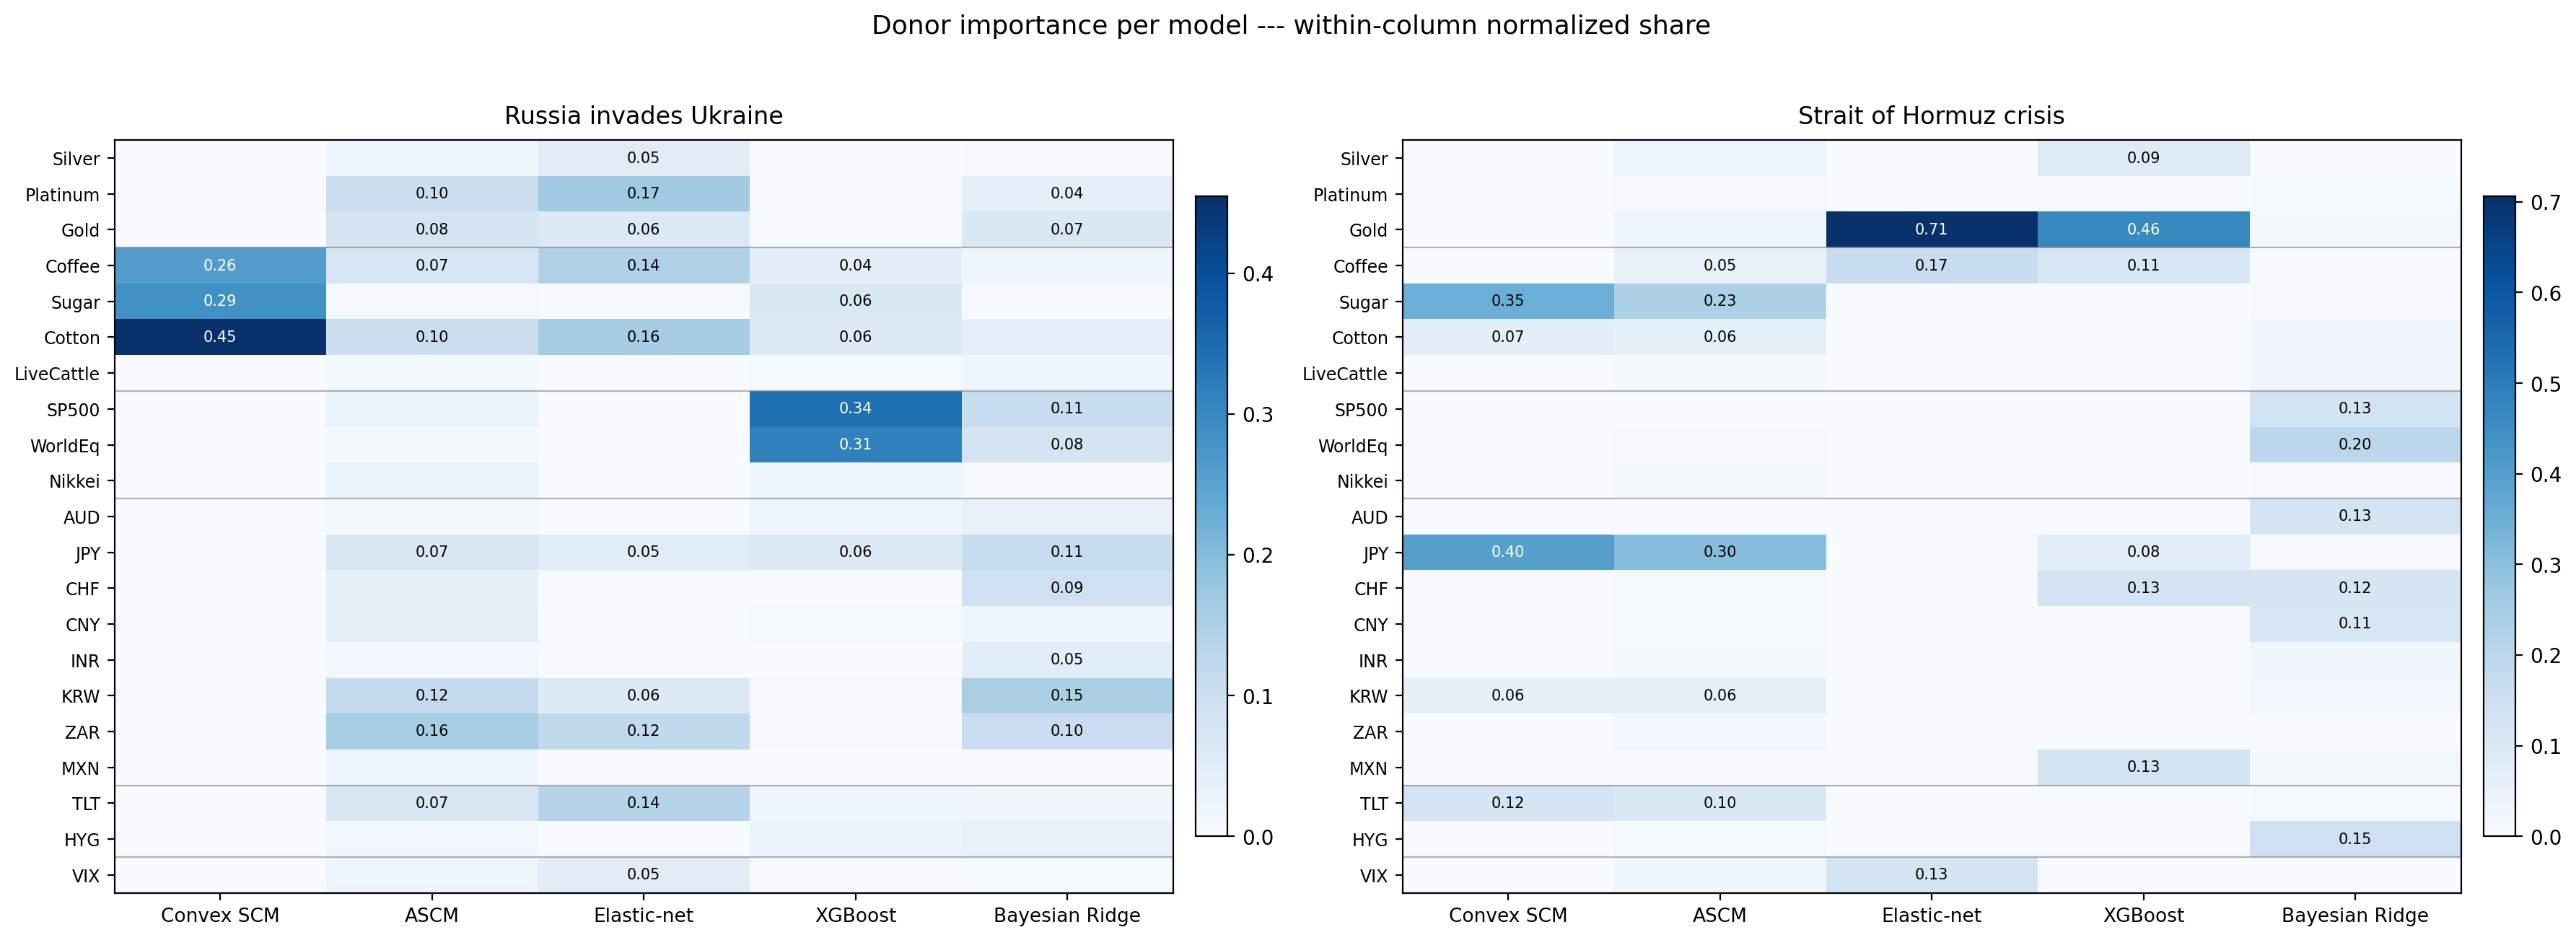
\includegraphics[width=\textwidth,height=0.70\textheight,keepaspectratio]{../../plots/milestone2/donor_importance_heatmap.png}
      \end{center}
    \end{column}
    \begin{column}{0.40\textwidth}
      \footnotesize
      \hd{Reading the heatmap.} Column-normalised donor importance per model
      (convex weight / $|\hat\beta_j|$ / feature importance).

      \vspace{0.5em}
      \hd{Hormuz.} Weight concentrates on \emph{safe-haven metals} (Gold, Platinum) and \emph{JPY / VIX}.
      These rose on generic risk but \emph{not} on the oil-specific shock $\rightarrow$ synthetic undershoots
      actual Brent $\rightarrow$ large \emph{positive} gap.

      \vspace{0.5em}
      \hd{Russia --- divergence is donor-driven.} The models split because they lean on \emph{different}
      donors: Convex/ASCM concentrate on Coffee \& Platinum ($w \approx 0.5$--$0.65$), XGBoost leans SP500
      ($\sim$0.48), while Bayesian Ridge blows up on JPY \& KRW ($w \approx 1.8$--$2.4$, far outside the
      simplex) $\rightarrow$ degeneracy. That is \emph{why} the ensemble IQR \emph{excludes} the two
      non-convex models.
    \end{column}
  \end{columns}
  \vspace{-0.2em}
  \begin{center}\smalltext{Per-model donor weights from data/validation/contamination\_bias\_top\_contributors.csv; concentration from donor\_concentration.csv.}\end{center}
\end{frame}

% =====================================================================
% COMMENT 2 (cont.) --- contamination bias is SIGNED and BOUNDED
% Directly answers the supervisor's demand-destruction critique.
% =====================================================================
\begin{frame}{Comment 2 --- the contamination bias is signed, and it makes us \emph{conservative}}
  \footnotesize
  \hd{The critique.} If high oil prices \emph{crowd out demand}, the donors that proxy global activity are
  themselves pushed \emph{down} by the treatment $\rightarrow$ the synthetic is dragged down with them
  $\rightarrow$ residual contamination in the gap. \hd{So: which way does the bias go, and how big?}

  \vspace{0.4em}
  \hd{We sign it.} For each linear model we decompose the gap into a clean component and a donor-contamination
  component (net bias) over the full post-window:

  \vspace{0.3em}
  \begin{center}
  \begin{tabular}{@{}l r r@{}}
    \toprule
    \hd{Model}     & \hd{Hormuz net bias} & \hd{Russia net bias} \\
    \midrule
    Convex SCM     & $-1.3\%$ \smalltext{(conservative)} & $+21.3\%$ \\
    ASCM           & $-2.3\%$ \smalltext{(conservative)} & $+11.8\%$ \\
    Elastic-net    & $-2.6\%$ \smalltext{(conservative)} & $+19.5\%$ \\
    Bayesian Ridge & $-7.3\%$ \smalltext{(conservative)} & $-7.5\%$ \\
    XGBoost        & \smalltext{n/a (nonlinear)}          & \smalltext{n/a (nonlinear)} \\
    \bottomrule
  \end{tabular}
  \end{center}
  \smalltext{Source: data/validation/contamination\_bias\_decomposition.csv.}

  \vspace{0.4em}
  \begin{itemize}\setlength\itemsep{0.1em}
    \item \hd{Hormuz: bias is \emph{negative} across all linear models} $\rightarrow$ the demand-destruction
      channel makes the SCM \emph{under}-state the premium. The headline \textcolor{accent}{\bfseries $\sim$59\%}
      is therefore a \hd{lower bound}, not an inflated one.
    \item \hd{Russia: bias is positive} ($+12$ to $+21\%$) $\rightarrow$ donors \emph{did} catch the invasion
      shock and drift up --- exactly the Russia-specific contamination we flagged, and why Russia is a
      magnitude check, not the headline.
  \end{itemize}
\end{frame}

% =====================================================================
% STATISTICAL TESTS --- (a) in-space placebo
% =====================================================================
\begin{frame}{Statistical test 1 --- in-space placebo}
  \footnotesize
  \hd{Procedure} \src{Abadie 2010}: refit the SCM treating each donor as treated; rank Brent's post/pre RMSPE
  ratio against the $N{=}20$ units (Brent $+$ 19 donors). \hd{Permutation $p = $ rank $/\,N$}; floor $p = 1/20 = 0.05$
  $\rightarrow$ rank 1 is the strongest signal the 19-donor pool can produce.

  \vspace{0.4em}
  \begin{center}
  \begin{tabular}{@{}l c c@{}}
    \toprule
                   & \hd{Hormuz 2026} & \hd{Russia 2022} \\
    \hd{Model}     & rank\,$\rightarrow$\,$p$ & rank\,$\rightarrow$\,$p$ \\
    \midrule
    Convex SCM     & \textbf{1\,$\rightarrow$\,0.05} & 10\,$\rightarrow$\,0.50 \\
    ASCM           & \textbf{1\,$\rightarrow$\,0.05} & 12\,$\rightarrow$\,0.60 \\
    Elastic-net    & \textbf{1\,$\rightarrow$\,0.05} & 8\,$\rightarrow$\,0.40  \\
    XGBoost        & \textbf{1\,$\rightarrow$\,0.05} & 4\,$\rightarrow$\,0.20  \\
    Bayesian Ridge & \textbf{1\,$\rightarrow$\,0.05} & 12\,$\rightarrow$\,0.60 \\
    \bottomrule
  \end{tabular}
  \end{center}
  \smalltext{Source: data/validation/inference\_inspace\_brent\_summary.csv (19-donor shared pool).}

  \vspace{0.4em}
  \begin{itemize}\setlength\itemsep{0.05em}
    \item \hd{Hormuz:} Brent ranks 1 for \hd{all five models} $\rightarrow$ its break beats every placebo; strongest signal the pool allows.
    \item \hd{Russia:} mid-pack (rank 8--12) for the linear models; XGBoost is best at rank 4 ($p{=}0.20$) but still not significant --- consistent with Russia as a magnitude check, not a clean inferential case.
  \end{itemize}
\end{frame}

% =====================================================================
% STATISTICAL TESTS --- (b) leave-one-out
% =====================================================================
\begin{frame}{Statistical test 2 --- leave-one-out (LOO)}
  \footnotesize
  \hd{Procedure.} Drop one influential donor ($w > 5\%$) at a time, refit, recompute the ATT. Report the
  \hd{range} (max $-$ min, pp) across the leave-one-donor-out refits --- a small range means no single donor
  drives the result.

  \vspace{0.5em}
  \begin{center}
  \begin{tabular}{@{}l r r@{}}
    \toprule
    \hd{Model}     & \hd{Hormuz LOO range (pp)} & \hd{Russia LOO range (pp)} \\
    \midrule
    Convex SCM     & $8.2$           & $26.8$          \\
    ASCM           & $\mathbf{5.7}$  & $19.1$          \\
    Elastic-net    & $6.7$           & $18.8$          \\
    XGBoost        & $6.1$           & $\mathbf{13.8}$ \\
    Bayesian Ridge & $10.4$          & $27.3\,\dagger$ \\
    \bottomrule
  \end{tabular}
  \end{center}
  \smalltext{Source: data/validation/inference\_loo\_\{event\}\_\{model\}.csv.}

  \vspace{0.4em}
  \begin{itemize}\setlength\itemsep{0.1em}
    \item \hd{Hormuz: tight} ($\sim$6--10 pp on a $\sim$59\% effect) --- no single donor flips the result; ASCM tightest.
    \item \hd{Russia: wide} (14--27 pp). Bayesian Ridge ($\dagger$ range crosses zero, $-21.9$ to $+5.4$) is
      LOO-fragile, consistent with its degenerate fit; XGBoost is the most stable. Reinforces Russia as a
      magnitude check, not the headline.
  \end{itemize}
\end{frame}

% (Breakpoint SUTVA test moved up into the Comment 1 section.)

% =====================================================================
% COMMENT 3 --- naive counterfactual comparison
% =====================================================================
\begin{frame}{Comment 3 --- naive counterfactual baselines}
  \footnotesize
  \hd{Question.} What does the donor-informed SCM buy us over baselines that ignore the donor pool entirely?
  We compare the ensemble-median SCM premium against four naive counterfactuals at the full post-window.

  \vspace{0.4em}
  \begin{center}
  \scriptsize
  \begin{tabular}{@{}l r r r r r@{}}
    \toprule
    \hd{Counterfactual}              & \hd{Hormuz \%} & \hd{Russia \%} & & & \\
    \midrule
    \hd{SCM ensemble (donor-informed)} & \textcolor{accent}{\hd{58.9}} & \textcolor{accent}{\hd{22.0}} & & & \\
    \midrule
    Random walk --- flat             & 51.9          & 8.7            & & & \\
    Random walk --- drift            & 52.6          & $-6.9$         & & & \\
    Linear trend                     & 73.8          & $-4.2$         & & & \\
    Interrupted time series (ITS)    & 73.8          & $-4.2$         & & & \\
    \bottomrule
  \end{tabular}
  \normalsize
  \end{center}
  \smalltext{Source: data/validation/naive\_baseline\_comparison.csv (full-window horizon).}

  \vspace{0.5em}
  \hd{Reading.}
  \begin{itemize}\setlength\itemsep{0.1em}
    \item \hd{Random walks understate} the premium --- they freeze the counterfactual at the last pre-event level
      and miss the donor-implied path the rest of the market was on.
    \item \hd{Linear trend / ITS overstate} Hormuz (74\%) and \emph{flip sign} on Russia ($-4\%$) --- naive
      extrapolation of a pre-trend is spurious when the donor factor itself turned.
    \item The SCM sits \hd{between} the two failure modes: anchored to a \emph{data-driven} counterfactual that
      tracks the global factor without freezing or blindly extrapolating it.
  \end{itemize}
\end{frame}

% =====================================================================
% Wrap-up
% =====================================================================
\begin{frame}{Summary --- headline ATT across post-event windows}
  \footnotesize
  \begin{enumerate}\setlength\itemsep{0.1em}
    \item[\textcolor{accent}{\hd{1}}] \hd{SUTVA} --- audit (oil-supply / disruption path), corroborated by the breakpoint test.
    \item[\textcolor{accent}{\hd{2}}] \hd{Model behaviour} --- weight on risk donors explains the gap; contamination bias signed (Hormuz conservative).
    \item[\textcolor{accent}{\hd{3}}] \hd{Naive baselines} --- random walks understate, trend / ITS over-extrapolate; the SCM sits between.
  \end{enumerate}

  \vspace{0.2em}
  \begin{center}
    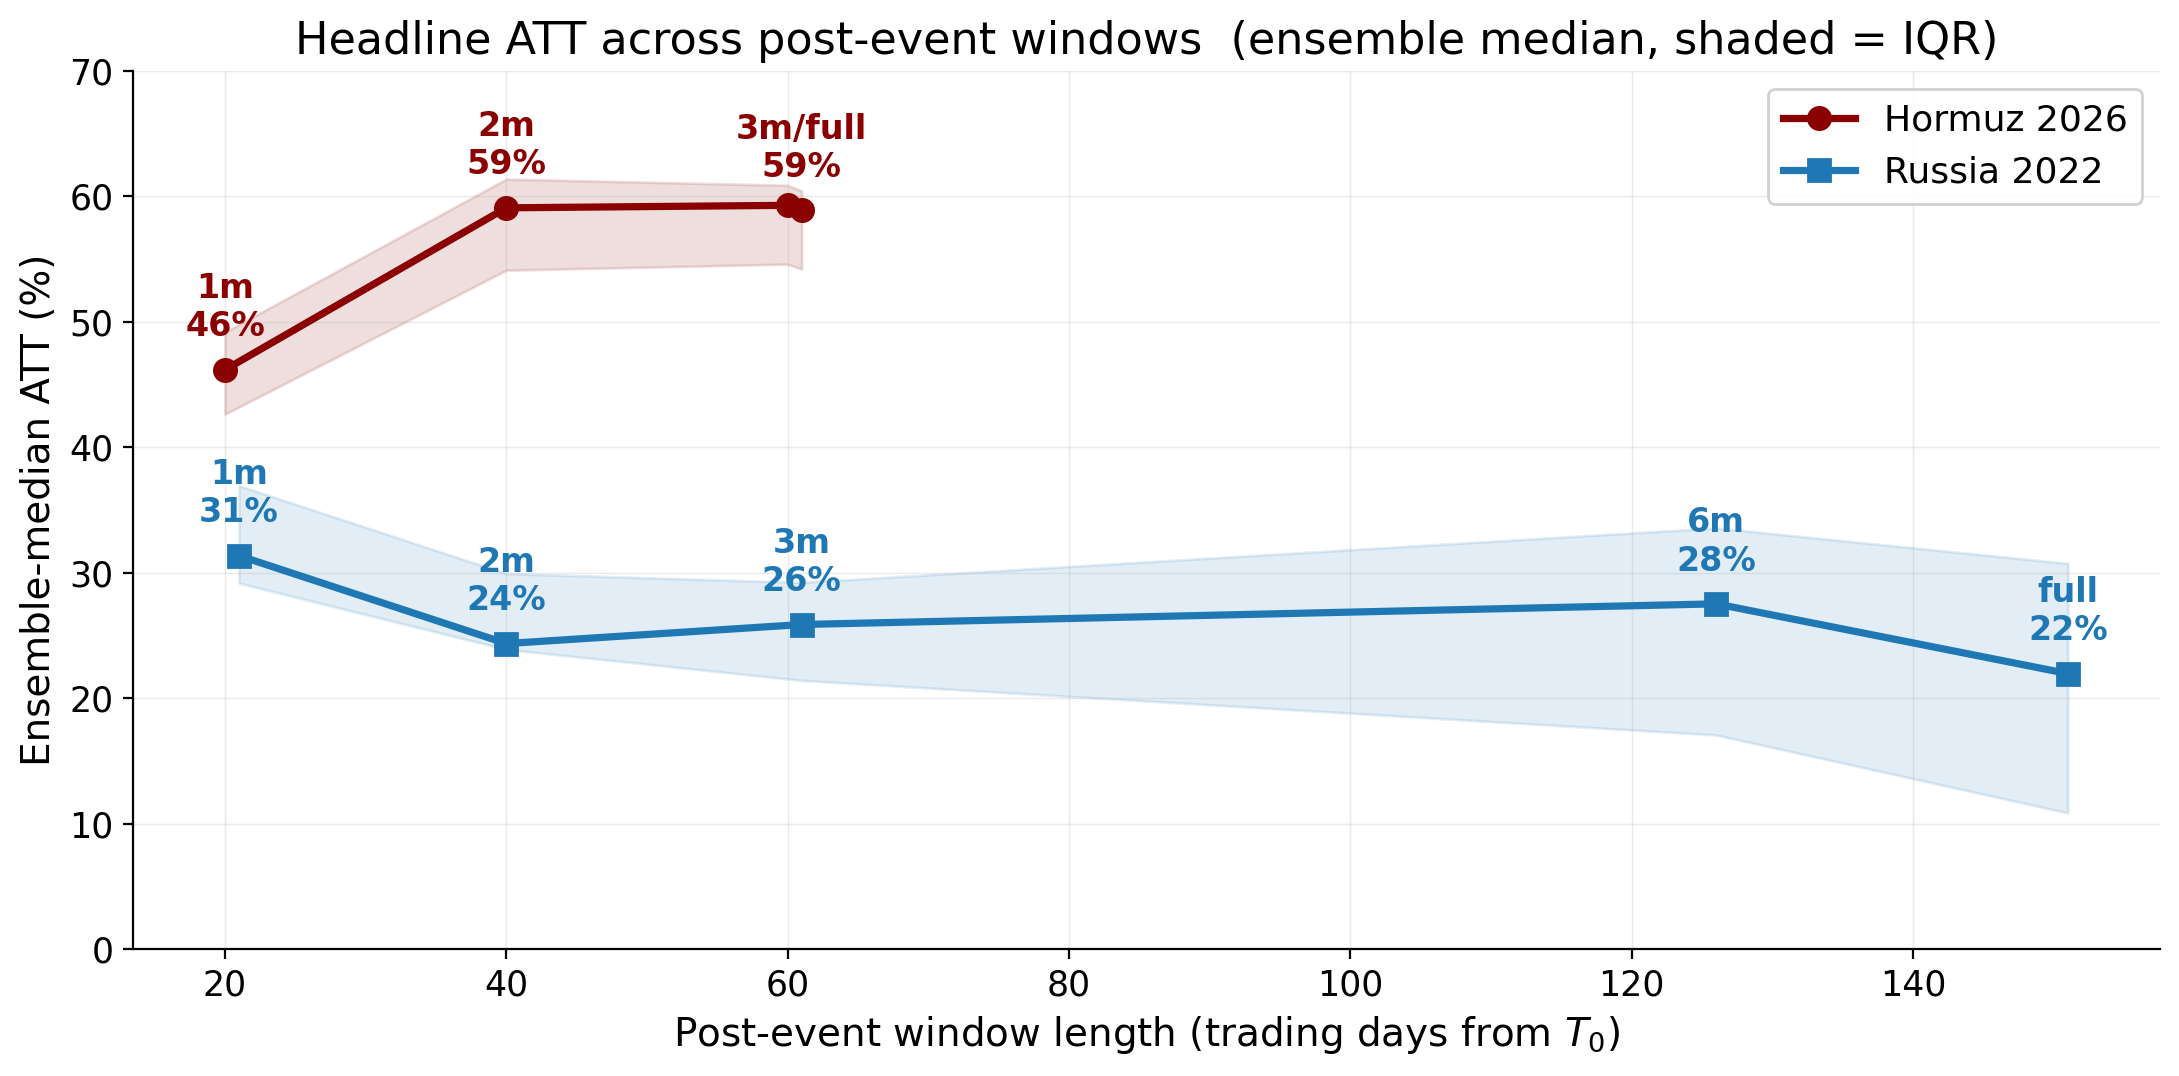
\includegraphics[width=0.78\textwidth,height=0.55\textheight,keepaspectratio]{../../plots/milestone3/postwindow_sensitivity.png}
  \end{center}

  \vspace{-0.3em}
  {\scriptsize \hd{Hormuz} builds to \textcolor{accent}{\hd{$\sim$59\%}} by month 2--3 and holds (IQR $[54,60]$);
  \hd{Russia} peaks $\sim$31\% (1m) and settles $\sim$22\% (full) --- the magnitude check.\par}
\end{frame}

% =====================================================================
% Closing
% =====================================================================
{\setbeamertemplate{footline}{}
\begin{frame}[plain]
  \vfill
  \begin{center}
    {\Large Thank you}\\[1em]
    {\normalsize Questions and discussion}\\[2em]
    \smalltext{github.com/ElvisCasco/Brent\_Analysis}
  \end{center}
  \vfill
\end{frame}
}

\end{document}
